 \chapter{Introduction}
 \label{introchap}
\section{Groundwater Contamination}
Below ground, water found in the spaces between soil, sand and rock
is called groundwater. It moves slowly through
\textbf{aquifers} as a function of pressure (\textbf{hydraulic head}), \textbf{porosity},
aquifer thickness, and aquifer \textbf{transmissivity}. Aquifers are
water-bearing layers of rock and sediments that hold
water~\cite{basics}. The pressure exerted on the groundwater is called
the hydraulic head. It is the sum of three components: the pressure
head, elevation head and velocity head~\cite{basics}. In other words,
the level that water entering a confined well will stand at is
determined by the hydraulic head. Porosity refers to the ratio of the empty
spaces to the total volume of the sediment; fine-grained materials tend to
have greater porosities than coarse-grained materials since they are
better sorted~\cite{basics}. Table~\ref{tbl:porosity} outlines typical
porosity ranges for three kinds of materials: clay, sand, and gravel.
\begin {table}[H]
\caption [Typical porosity ranges for clay, sand, and gravel]{Typical
  porosity ranges for clay, sand, and gravel~\cite{basics}.} \label{tbl:porosity}
\begin{center}
    \begin{tabular}{ | c | c | c |}
    \hline
    Grain Size & Material & Porosity \\ \hline
    Fine & Clay  &  50\% \\ \hline
    Medium &  Sand & 25\% \\ \hline
    Coarse &  Gravel &  20\% \\ \hline
    \end{tabular}
\end{center}
\end{table}
\noindent Transmissivity characterizes the volume of water flowing through a
 cross-section of the aquifer (1 ft. by the aquifer thickness), under
 a hydraulic gradient of 1 ft./ 1 ft. per unit of time (usually one day)~\cite{basics}.

Groundwater is vital
to providing drinking water, irrigation, and makes up a large
component in many industrial processes. Figure~\ref{fig:gwuse}
demonstrates how groundwater is used in the United States. 
\begin{figure}[!h]
\caption[Groundwater usage in the United States in 2005]{The total
  groundwater withdrawls in the United States in 2005 is categorized
  in terms of use~\cite{usgsgw}.}\label{fig:gwuse}
    \begin{center}
	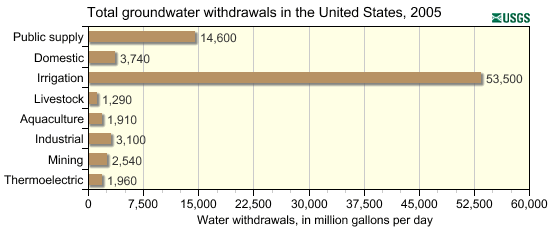
\includegraphics[scale=0.8]{figs/gwuse.png}
    \end{center}
\end{figure}
Most
notably, about 51\% of the total U.S. population and 99\% of the
rural population rely on groundwater as their drinking water
source~\cite{gw}. Unfortunately, by nature of being underground,
groundwater is highly susceptible to contaminants, e.g. fertilizers,
pesticides, road salt, gasoline, etc. Toxins that have leached into
the water supply have deleterious effects on human health as well as
serious environmental ramifications. 

We explore the characteristics of spatially perturbed one-dimensional
maps with the aim of understanding \textbf{in situ remediation} of contaminated
groundwater. In situ remediation involves injecting a treatment
solution in the groundwater to render the contaminants
inert. Degredation reactions require the two solutions be in close proximity to each other; the solutions must mix. Engineered Injection and Extraction (EIE)\footnote{EIE sequences are typically developed
heuristically to stretch and fold the fluid interface.} is an
approach that uses sequential injection and extraction of water in wells surrounding
the contaminated region to generate chaotic \textbf{advection}. A
solute is advected through a system when it moves with the local fluid
velocity~\cite{advection}. Degredation reactions are more efficient when the solutions are thoroughly mixed
together, so the onset of chaos in this system is a positive sign
because it indicates the interface length between the two reactants is
maximal. The primary agents of mixing are the local velocity
variations due to aquifer heterogeneity and the extent to which
solutions move underground (transmissivity)
\cite{neupauer}. Therefore, the spatial distribution of rocks and
sediment plays an important role in the dynamics of the system. 

Exploring the dynamics of a one-dimensional system lays the groundwork
for understanding the dynamics of systems with higher dimensions. Two
one-dimensional systems known to exhibit chaotic behavior are the
logistic map and the circle map. Applying spatial perturbations to
these maps and observing the subsequent dynamics may give an
indication of what occurs in two-dimensional systems, like the
groundwater model. 

\section{Chaos}
One-dimensional maps, such as the logistic map and the circle map, are
analyzed in a variety of ways, e.g. fixed point iterations,
cobweb diagrams, bifurcation diagrams, etc. This section offers some
basic definitions and explanations of these concepts. One-dimensional Maps are a
subclass of dynamical systems in which time is discrete, rather than
continuous. They take the form
\begin{equation*}
x_{n+1}=f(x_n).
\end{equation*}
These maps demonstrate that even simple dynamical systems are capable
of complex behavior, and as such, are also simple examples of
\textbf{chaos}. Although no universal definition of chaos has been
agreed upon, the following working definition is generally acceptable~\cite{strogatz}:
\begin{singlespace}
\begin{definition}
Chaos is aperiodic long-term behavior in a deterministic
  system that exhibits sensitive dependence on initial conditions.
\end{definition}
\end{singlespace}
\begin{enumerate}
\item \textbf{Aperiodic long-term behavior} is another way of stating
  that there are trajectories within the map that do not limit to
  fixed points or more generally quasiperiodic orbits as $n \to \infty$.
\item \textbf{Deterministic} is used to describe systems in which
  there is no random input or parameter. The observed behavior of the
  system arises from its nonlinearity, not from random noise.
\item \textbf{Sensitive dependence on initial conditions} means that
  trajectories that start in almost the same place ($\epsilon$ apart)
  separate quickly. In other words, the system has a
  positive Lyapunov exponent.
\end{enumerate}

The sequence of iterates ${x_0,x_1,...,x_n}$ in a map is
called an \textbf{orbit}. As $n \to \infty$, orbits may converge on a fixed point, or a
set of fixed points. A \textbf{fixed point} $x^*$ of a function $f$ is an element of the
function's domain that is mapped to itself by the function, i.e.
\begin{equation*}
x^* = f(x^*).
\end{equation*}
The stability of the fixed point $x^*$ is
determined by perturbing the fixed point by $\eta$ to see whether it is
attracted to or repelled from $x^*$. A Taylor series expansion around
the perturbation $x_{n+1} = x^* + \eta_{n+1}$ linearizes the map
\begin{align*}
\begin{split}
x_{n+1} &= x^* + \eta_{n+1}\\
x^* + \eta_{n+1} &= f(x^* + \eta_n)\\
&= f(x^*) + f'(x^*)\eta_n + \mathcal{O}(\eta_n^2),\\
\eta_{n+1} &= f'(x^*)\eta_n + \mathcal{O}(\eta_n^2).\\
\end{split}
\end{align*}
Neglecting the higher order terms in $\mathcal{O}(\eta_n^2)$ leaves
$\eta_{n+1} = f'(x^*)\eta_n$. The multiplier is $\hat{\lambda} =
f'(x^*)$. Solutions of the map are found by extending the recursion
\begin{align*}
\begin{split}
\eta_{1} &= \hat{\lambda}\eta_0\\
\eta_{2} &= \hat{\lambda}\eta_1 = \hat{\lambda}^2\eta_0\\
&...\\
\eta_{n} &=\hat{\lambda}^n\eta_0.
\end{split}
\end{align*}
If $|\hat{\lambda}| = |f'(x^*)| > 1$, $\lim_{n \to \infty}\hat{\lambda}^n = \infty$, and
the fixed point $x^*$ is \textbf{linearly unstable}. If $|\hat{\lambda}| = |f'(x^*)| < 1$, $\lim_{n \to
  \infty}\hat{\lambda}^n = 0$, and the fixed point $x^*$ is
\textbf{linearly stable}. If
$|\hat{\lambda}| = |f'(x^*)| = 1$ the $\mathcal{O}(\eta_n^2)$ terms
determine the local stability~\cite{strogatz}. Linear stability is
linked to nonlinear stability by the Hartman-Grobman Theorem~\cite{meiss}.
\begin{singlespace}
\begin{theorem}
Hartman-Grobman Theorem: Let $x^*$ be a hyperbolic equilibrium point of a $C^1$
vector field $f(x)$ with flow $\phi_t(x)$. Then there is a
neighborhood $N$ of $x^*$ such that $\phi$ is topologically conjugate to its linearization on $N$.
\end{theorem}
\end{singlespace}
The Hartman-Grobman theorem states the behavior of the linearized
dynamical system near a fixed point is equivalent to the
behavior of the nonlinear system near the same point, as long as the
multiplier $|\hat{\lambda}|\neq 1$. Therefore, the results of linear stability
analysis of fixed points translates to nonlinear stability. 

A \textbf{cobweb diagram} is a graphical representation of the orbit
iterations. The method of the cobweb diagram can be outlined in four
steps, and is depicted in Figure~\ref{fig:cobex}:
\begin{enumerate}
\item Begin at the Cartesian coordinate pair $(x_0, f(x_0))$, which
  may also be written as $(x_0, x_1)$
\item Plot horizontally the distance from $(x_0, f(x_0)=(x_0, x_1)$ to $(f(x_0),
  f(x_0))=(x_1, x_1)$
\item Plot vertically from $(f(x_0), f(x_0))=(x_1, x_1)$ to $(f(x_0), f(f(x_0)))=(x_1, x_2)$
\item Repeat steps 2-3 until convergence or divergence is determined:
  $(x_n, x_{n+1}) \to (x_{n+1}, x_{n+1}) \to (x_{n+1},x_{n+2})$
\end{enumerate}
\begin{figure}[!h]
\caption[Example of a Cobweb Diagram]{A One-dimensional Map (blue) and
  the line $x_{n+1}=x_n$ (red) with a few iterates of the cobweb
  diagram (green). Cobweb diagrams encapsulate the dynamics of the orbit at a glance.}\label{fig:cobex}
    \begin{center}
	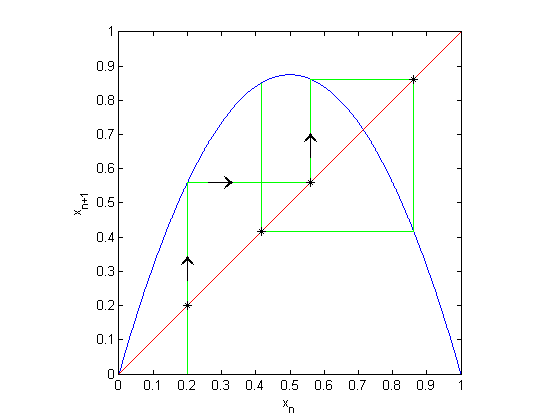
\includegraphics[scale=0.8]{figs/cobweb_ex.png}
    \end{center}
\end{figure}

\textbf{Lyapunov exponents} are a way of classifying a the sensitive
dependence on initial conditions for a specific orbit. They are
defined as 
\begin{equation}
\lambda(x_0) = \lim_{n \to \infty} \frac{1}{n} \sum_{i=0}^{n-1} \ln |f'(x_i)|.
\end{equation}
$\lambda(x_0)$ is the same for all initial conditions $x_0$ in the same \textbf{basin of
attraction}. The basin of attraction for an attracting fixed point
$x^*$ is defined as the set $S=\{x_0:x(t) \to x^*, t \to \infty\}$, i.e.
the set of initial conditions $x_0$ that are drawn to the fixed point
as time goes to infinity~\cite{strogatz}. For stable fixed points and periodic orbits, $\lambda(x_0) < 0$,
and for chaotic attractors, $\lambda(x_0)>0$.


% For example, a common problem is to insert graphics ---
% figures and tables --- into the body of the thesis.  For
% this one should use the {\tt graphicx} package, which is
% part of the standard \TeX{} distribution.  Likewise, the
% Grad School specs say that a large table may be displayed
% in landscape mode at reduced size, but its caption must
% also be in rotated position, in the same font and size as
% the normal text in the body of the thesis.  To accomplish
% this, the user must invoke the {\tt rotating} package,
% available online.


% \section{Lists in {\tt thesis} class}

% In {\tt thesis} class (for Colorado University),
% lists are defined so that nested lists will be
% numbered or marked appropriately.
% First, an itemized (non-enumerated) list
% prefaces each item with a bullet.
% Nested itemized list use asterisks,
% then dashes, then dots.
% These lists are typed between
% the \verb2\begin{itemize}2
% and \verb2\end{itemize}2
% commands.

% \begin{itemize}
%   \item{} This is ``itemized'' item A.
%   \item{} This is ``itemized'' item B.
%   \item{} This is ``itemized'' item C.
%   \begin{itemize}
%     \item{} This is ``itemized'' subitem A.
%     \begin{itemize}
%       \item{} This is ``itemized'' subsubitem A.
%       \begin{itemize}
%         \item{} This is ``itemized'' subsubsubitem A.
%       \end{itemize}
%       \item{} This is ``itemized'' subsubitem B.
%     \end{itemize}
%     \item{} This is ``itemized'' subitem B.
%   \end{itemize}
%   \item{} This is ``itemized'' item D.
% \end{itemize}

% Enumerated lists use the commands
% \verb2\begin{enumerate}2 and
% \verb2\end{enumerate}2,
% and nested enumerations appear like this.

% \begin{enumerate}
%   \item{} This is ``enumerated'' item A.
%   \item{} This is ``enumerated'' item B.
%   \item{} This is ``enumerated'' item C.
%   \begin{enumerate}
%     \item{} This is ``enumerated'' subitem A.
%     \begin{enumerate}
%       \item{} This is ``enumerated'' subsubitem A.
%       \begin{enumerate}
%         \item{} This is ``enumerated'' subsubsubitem A.
%       \end{enumerate}
%       \item{} This is ``enumerated'' subsubitem B.
%     \end{enumerate}
%     \item{} This is ``enumerated'' subitem B.
%   \end{enumerate}
%   \item{} This is ``enumerated'' item D.
% \end{enumerate}


% The work presented
% here\footnote{Footnotes are handled neatly by \LaTeX.}
% is an extension of Lao\cite{lao:thesis}
% and Lao et~al.\cite{lao:paper},
% fictional references that are in the bibliographic
% source file \verb9refs.bib9.

% \begin{table}[htb]
%     \caption[Example of a table with its own footnotes]{
% 	Here is an example of a table with its own footnotes.
% 	Don't use the $\backslash${\tt footnote} macro if you
% 	don't want the footnotes at the bottom of the page.
% 	Also, note that in a thesis the caption goes
% 	\emph{above} a table, unlike figures.
% 	}
%     \begin{center}
%     \begin{tabular}{||l|c|c|c|c||} \hline
% 	& $S$ & $P$ &   $Q^{\ast}$  & $D^{\dagger}$ \\	% footnote symbols!
% 	wave form & (kVA) & (kW) & (kVAr) & (kVAd) \\  \hline \hline
% 	Fig.  \ref{xfigDiagram}a  & 25.48 & 25.00 & -2.82 & 4.03 \\ \hline
% 	Fig.  \ref{xfigDiagram}b  & 25.11 & 18.02 & -9.75 & 14.52 \\ \hline
% 	Table \ref{pdftable}  & 24.98 & 22.26 & 9.19 & 6.64 \\ \hline
% 	Table \ref{powertable}  & 23.48 & 15.00 & 6.59 & 16.82 \\ \hline
% 	Fig.  \ref{pyramid}  & 24.64 & 22.81 & -0.44 & 9.3 \\ \hline
% 	\end{tabular}
%    \\ \rule{0mm}{5mm}
%    ${}^\ast$kVAr means reactive power.		% footnote symbol
% \\ ${}^\dagger$kVAd means distortion power.	% footnote symbol
% \end{center}
% \label{powertable}
% \end{table}


